\selectlanguage{british}%

\chapter{Contextuality and Bohmian Mechanics}


\section{Rationale}

We saw in the last chapter that BM is able to explain the GHZ test.
The paradox arises if we try to multiply values assigned to operators
that don't commute, to obtain the value assigned to a product of such
operators. In BM, since the operator must be provided to obtain it's
value, no contradiction arises, even though the results are deterministic
(given all initial conditions). %
\begin{comment}
Effectively then, at the risk of repetition, the flaw in our GHZ reasoning,
was that we were commuting operators that didn't commute, by assuming
they were numbers.
\end{comment}
Thus, we were only able to rule out theories that treated operators
like numbers and we find that BM is not one of them. However, as we
have seen in the Peres Mermin (PM) test, the operators whose values
are multiplied, do infact commute, implying that the PM test is exonerated
from that objection. And we also know that BM, atleast on the face
of it, is non-contextual, viz. the value obtained upon the measurement
of an operator, depends only on the state (+ hidden variables) and
the operator, granted we fix our measurement scheme. It is therefore
not clear how BM is contextual, which is a notion we're forced to
accept from the PM test. Further, since BM is claimed to reproduce
all results of QM, does it entail that a non-contextual theory can
explain the PM test?

We also found in the previous chapter, that in BM, there's no fundamental
difference that arises between the phase space variables and spins.
As we saw, the value of momentum observed, depends on the systematics
of the measurement process, just as the outcome of a spin measurement
using an SG setup (as was discussed in the first chapter). Therefore
in what follows, attempts will be made at tackling the problem from
whichever method, (between phase space and spins) appears more accessible. 


\section{Intensifying Contextuality}

We have already seen that GHZ test is a test of determinism, of whether
predefined values can explain QM, while the PM test is that of contextuality,
which says that predefined non-contextual values, a more subtle remark,
can't explain QM. We also learnt how one can extend the GHZ test to
continuous variables. In this section, we will make both these schemes
effectively equally powerful; make GHZ into a test of contextuality
and extend the PM test to continuous variables. 


\subsection{GHZ escalated to Contextuality \label{sub:GHZ-to-contextuality}}

Recall from the first chapter, $\hat{A}\equiv\sigma_{x}\otimes\sigma_{y}\otimes\sigma_{y}$,
$\hat{B}\equiv\hat{\sigma}_{y}\otimes\hat{\sigma}_{x}\otimes\hat{\sigma}_{y}$,
$\hat{C}\equiv\hat{\sigma}_{y}\otimes\hat{\sigma}_{y}\otimes\hat{\sigma}_{x}$
and $\hat{D}=\hat{\sigma}_{x}\otimes\hat{\sigma}_{x}\otimes\hat{\sigma}_{x}$,
and $\hat{A}\hat{B}\hat{C}=-\hat{D}$. Consider now, in addition,
the following operators, 
\[
\hat{H}_{ij}\doteq\left[\begin{array}{ccc}
\hat{\sigma}_{x}\otimes\hat{\mathbb{I}}\otimes\hat{\mathbb{I}}^{(a)} & \hat{\mathbb{I}}\otimes\hat{\sigma}_{y}\otimes\hat{\mathbb{I}}^{(2)} & \mathbb{\hat{I}}\otimes\mathbb{\hat{I}}\otimes\hat{\sigma}_{y}^{(3)}\\
\hat{\sigma}_{y}\otimes\mathbb{\hat{I}}\otimes\hat{\mathbb{I}}^{(1)} & \hat{\mathbb{I}}\otimes\hat{\sigma}_{x}\otimes\hat{\mathbb{I}}^{(b)} & \mathbb{\hat{I}}\otimes\hat{\mathbb{I}}\otimes\hat{\sigma}_{y}^{(3)}\\
\hat{\sigma}_{y}\otimes\mathbb{\hat{I}}\otimes\hat{\mathbb{I}}^{(1)} & \mathbb{\hat{I}}\otimes\hat{\sigma}_{y}\otimes\hat{\mathbb{I}}^{(2)} & \mathbb{\hat{I}}\otimes\hat{\mathbb{I}}\otimes\hat{\sigma}_{x}^{(c)}\\
\hat{\sigma}_{x}\otimes\mathbb{\hat{I}}\otimes\hat{\mathbb{I}}^{(a)} & \mathbb{\hat{I}}\otimes\hat{\sigma}_{x}\otimes\hat{\mathbb{I}}^{(b)} & \hat{\mathbb{I}}\otimes\hat{\mathbb{I}}\otimes\hat{\sigma}_{x}^{(c)}
\end{array}\right]
\]
and note that (a) the product of these operators along each row, yields
$\hat{A}$, $\hat{B}$, $\hat{C}$ and $\hat{D}$ respectively, (b)
operators along any row, commute and (c) the superscript labels identify
operators that are repeated. 

We will now try to assign values to $\hat{H}_{ij}$ and only multiply
values assigned to commuting observables, to obtain the value of $\hat{A},\hat{B},\hat{C}$
and $\hat{D}$. We know (see \prettyref{sec:Determinism-The-GHZ})
that according to QM, for the GHZ state, $\left|\chi_{G}\right\rangle $,
$\hat{A},\,\hat{B}$ and $\hat{C}$ must be assigned the value $+1$,
while $\hat{D}$ must be assigned $-1$. We demand that our assignment
corresponds to this state. Let us start with assigning values to the
last row. To obtain a $-1$ corresponding to $D$, we must have either
a $1,1,-1$ (or permutations) or $(-1,-1,-1)$. Let us assume that
the former is true. At this stage then, we'd have 
\[
H_{ij}\doteq\left[\begin{array}{ccc}
1\\
 & 1\\
 &  & -1\\
1 & 1 & -1
\end{array}\right].
\]
Now to obtain a $+1$ in the first row (for $A$), we must have $(1,\pm1,\pm1)$.
Similarly we get, for the second row, $(\pm1,1,\pm1)$. The assignment
then becomes 
\[
H_{ij}\doteq\left[\begin{array}{ccc}
1 & \pm1 & \pm1\\
\pm1 & 1 & \pm1\\
\pm1 & \pm1 & -1\\
1 & 1 & -1
\end{array}\right],
\]
however, we have no freedom left and are forced to assign $-1$ to
the third row, while we were required to have it equal $+1$. A little
reflection reveals that the $(-1,-1,-1)$ case for the last row, won't
resolve the issue. Thus we conclude that the assignment must be contextual
(atleast the one corresponding to $\left|\chi_{G}\right\rangle $).
In this scenario, the non-commuting observables argument, deduced
in the previous chapter fails. Here, values of only commuting observables
were multiplied, even though effectively it is still the same GHZ
test.


\subsection{Peres Mermin escalated to Continuous Variables \label{sub:Peres-Mermin-phaseSpace}}

The Peres Mermin situation can be, quite simply, extended to continuous
variables, which maybe of practical interest. Performing SG type setup
in the simulation requires implementation of spins and appropriate
magnetic field effects, and that can be surpassed with this construction.
To this end, the following extension was worked out (but this result
was already known \cite{contextualityPhaseSpace}). For any unitary
operators $\hat{X}$ and $\hat{Y}$, s.t. $\{\hat{X},\hat{Y}\}=0$
and so is $\{\hat{X},\hat{Y}^{\dagger}\}=0$, if we define $\hat{Z}=i\hat{Y}\hat{X}$,
then 
\[
\begin{array}{ccc}
\hat{X}\otimes\hat{\mathbb{I}} & \hat{\mathbb{I}}\otimes\hat{X} & \hat{X}^{\dagger}\otimes\hat{X}^{\dagger}\\
\hat{\mathbb{I}}\otimes\hat{Y} & \hat{Y}\otimes\hat{\mathbb{I}} & \hat{Y}^{\dagger}\otimes\hat{Y}^{\dagger}\\
\hat{X}^{\dagger}\otimes\hat{Y}^{\dagger} & \hat{Y}^{\dagger}\otimes\hat{X}^{\dagger} & \hat{Z}\otimes\hat{Z}
\end{array}
\]
would yield the PM situation. To check this, note that the product
along any row, is $\hat{\mathbb{I}}$ and it is also so for each column,
except for the third, which is $-\hat{\mathbb{I}}$, precisely the
same as the PM situation. The difference however, will be that the
corresponding hidden variables, will have to be unimodular complex
(viz. $XX^{*}=1$) and the values of the operators, must be deduced
from their hermitian counterparts. One such choice of $X$ and $Y$
was pointed out in the previous chapter; $\hat{X}\equiv e^{i\sqrt{\pi}\hat{q}/\hbar L}$
and $\hat{Y}\equiv e^{i\sqrt{\pi}\hat{p}L/\hbar}$. Note that in this
case, optimization is not required, for this test is state independent
(should work with any choice of states).


\section{Measurements in BM (II)}

Measurements have already been discussed at length in the previous
chapters, however, we are now particularly interested in measuring
spins, especially when there is entanglement. We will see how a measurement
made using the Stern Gerlach like apparatus can yield results very
different from those obtained by the Hamiltonian approach. Further,
we will see how the former can get difficult to evaluate, quite quickly.


\subsection{Stern Gerlach based measurements \label{sub:BM-entangled-Stern-Gerlach}}

Since we have already discussed how to analyse a Stern Gerlach based
measurement for a single particle, let us try to explore how to analyse
this for $\left|\chi\right\rangle =\left|++\right\rangle +\left|--\right\rangle /\sqrt{2}$,
where for instance $\left|++\right\rangle =\left|+\right\rangle _{A}\otimes\left|+\right\rangle _{B}$
($A$ and $B$ label the particle), and $\hat{\sigma}_{x}\otimes\hat{\sigma}_{x}$
is the observable of interest. Borrowing the notation and the analysis
from \prettyref{sec:Bohm's-Theory,-Bohmian}, we have $\sqrt{2}\left|\Psi_{S}\right\rangle =\left|\psi,\psi\right\rangle \otimes\left[\left|++\right\rangle +\left|--\right\rangle \right]$
initially and after the interaction, $\sqrt{2}\left|\Psi_{S}(t)\right\rangle =\left|\psi_{at},\psi_{at}\right\rangle \otimes\left|++\right\rangle +\left|\psi_{-at},\psi_{-at}\right\rangle \otimes\left|--\right\rangle $,
where $\left|\psi_{at},\psi_{at}\right\rangle =\left|\psi_{at}\right\rangle _{A}\otimes\left|\psi_{at}\right\rangle _{B}$
for example. Now, we must predict the outcome, given the initial positions
of the particles. We then plot $P(q_{1},q_{2})=\left\langle \Psi_{S}|q_{1},q_{2}\right\rangle \left\langle q_{1},q_{2}|\Psi_{S}\right\rangle $,
where $q_{1}$ and $q_{2}$ represent the $z$ coordinate of the particles,
and effectively we are summing over the spin degree of freedom, asking
for the probability of finding the particles near $q_{1}$ and $q_{2}$.
Initially, $P=\left|\left\langle q_{1},q_{2}|\psi,\psi\right\rangle \right|^{2}$
which would yield circles in a contour plot (showing say 70\% probability
enclosed within), see \prettyref{fig:sgMeas-Initial-State}. 
\begin{figure}
\begin{centering}
\subfloat[Initial State \label{fig:sgMeas-Initial-State}]{\begin{centering}
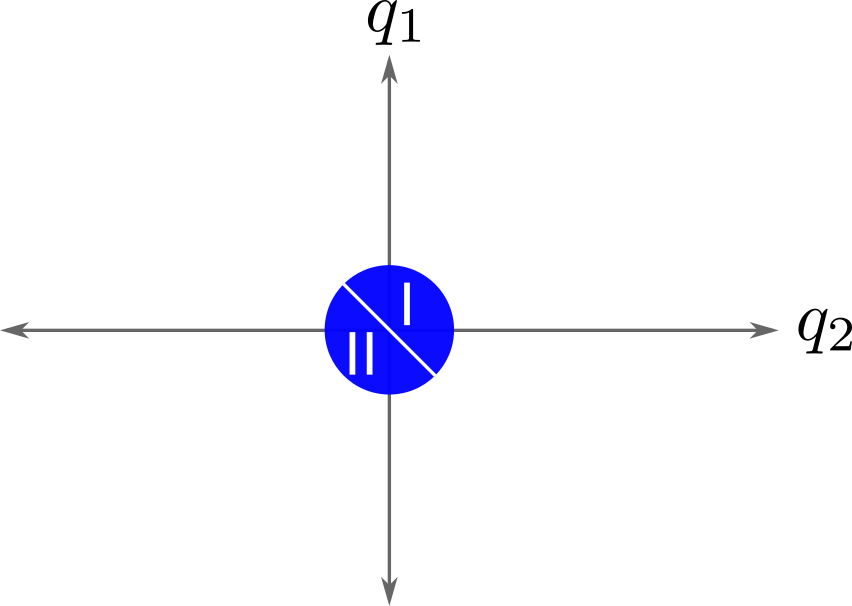
\includegraphics[width=0.3\columnwidth]{Chapter3/Figs/Raster/initial}
\par\end{centering}



\selectlanguage{english}%
\selectlanguage{english}%
}\subfloat[For $\sqrt{2}\left|\chi\right\rangle =\left|00\right\rangle +\left|11\right\rangle $\label{fig:sgMeas-Entangled}]{\begin{centering}
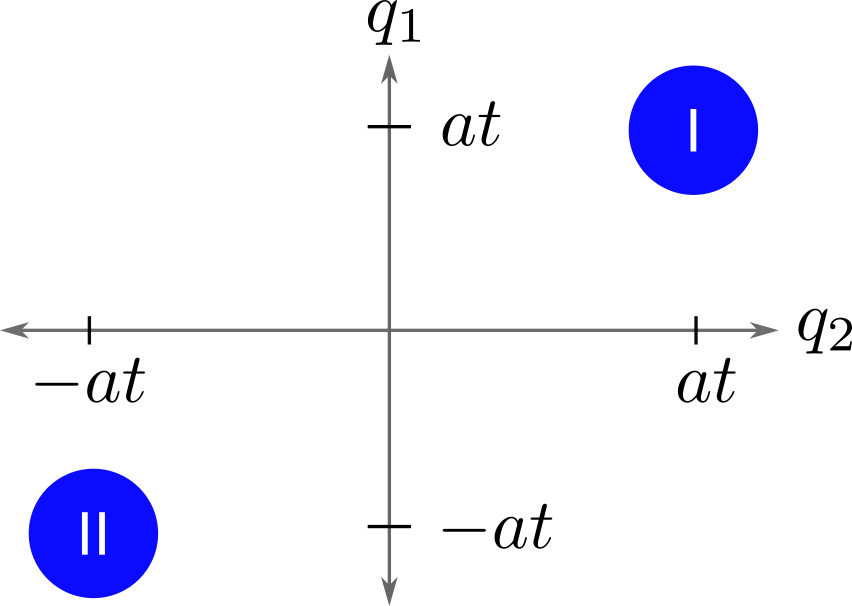
\includegraphics[width=0.3\columnwidth]{Chapter3/Figs/Raster/finalEntangled}
\par\end{centering}



\selectlanguage{english}%
\selectlanguage{english}%
}\subfloat[For $\left|\chi\right\rangle =\left|++\right\rangle $\label{fig:sgMeas-++}]{\begin{centering}
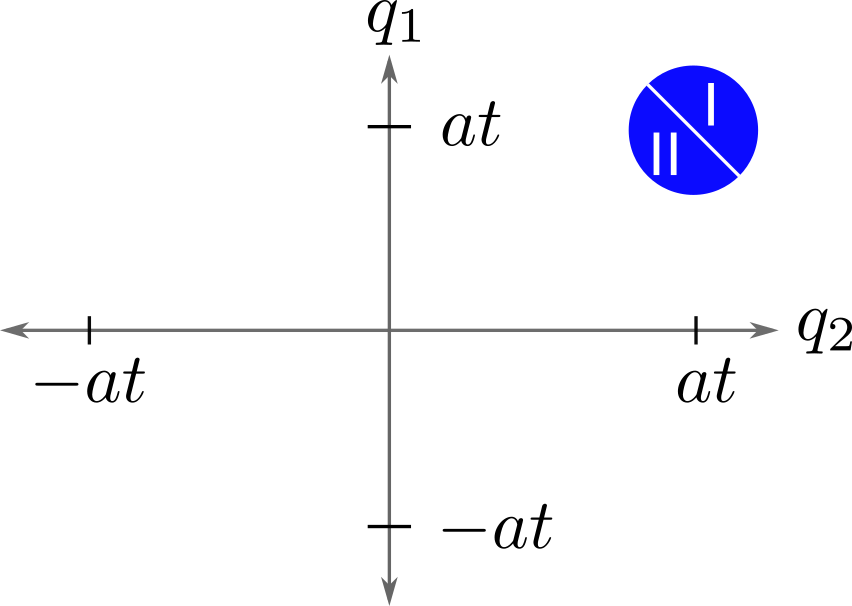
\includegraphics[width=0.3\columnwidth]{Chapter3/Figs/Raster/final}
\par\end{centering}

}
\par\end{centering}

\caption{Indicative contour plots for $\left|\left\langle q_{1},q_{2}|\Psi_{S}\right\rangle \right|^{2}$,
illustrating spin measurement of 2 particles, using the Stern Gerlach
setup.}


\selectlanguage{english}%
\selectlanguage{english}%
\end{figure}
After the interaction, $2P(q_{1},q_{2})=\left|\left\langle q_{1},q_{2}|\psi_{at},\psi_{at}\right\rangle \right|^{2}+\left|\left\langle q_{1},q_{2}|\psi_{-at},\psi_{-at}\right\rangle \right|^{2}$,
which would yield two circles in the countour plot, one centred at
$(at,at)$ and the other centred at $(-at,-at)$, see \prettyref{fig:sgMeas-Entangled}.
From the symmetry of the problem, and from the fact that velocities
are single valued, we can deduce that if the particle positions were
represented by a point inside area $I$, then the result would be
a spin up, viz. $\left|+\right\rangle $ for both, while for the other
case, the result would be spin down for both. Note that there's no
initial condition for which the results are anti-correlated, consistent
with $\left|\chi\right\rangle $. Although it is obvious, it is instructive
to see how this would work for $\left|\chi\right\rangle =\left|++\right\rangle $
for instance. In this case also, the initial plot for $P$ is identical
to that shown in \prettyref{fig:sgMeas-Initial-State}. However, since
after the interaction, $\left|\Psi_{S}(t)\right\rangle =\left|\psi_{at},\psi_{at}\right\rangle \otimes\left|++\right\rangle $,
we see that $P=\left|\left\langle q_{1},q_{2}|\psi_{at},\psi_{at}\right\rangle \right|^{2}$,
which is just a Gaussian centred at $(at,at)$, as shown in \prettyref{fig:sgMeas-++}.
Now, regardless of the initial conditions of the particles, after
the interaction, they will be carried to a Gaussian at $(at,at)$
by the probability current (which is effectively their velocity).
Thus, the result is always spin up, for both particles, consistent
with QM.

It is straight forward to extend this analysis to the GHZ situation,
with three particles. However, in that case, determining which area
(in phase space, viz. the set of initial positions) corresponds to
which outcome, becomes non-trivial, for certain operators. The difficulty
arises from the increasing possible final states. 


\subsection{Hamiltonian Approach\label{sub:BM-Hamiltonian-Approach-Spins}}

We have already used the Hamiltonian approach in \prettyref{sec:Measurements-in-BM}
and so extending it to spins will not be surprising. However, as we
will see, it incredibly simplifies the measurement process.


\subsubsection{Single Spin\label{sub:HamiltonianMeasureSingle-Spin}}

Let the spin state of our particle, be $\sqrt{2}\left|\chi\right\rangle =\left|0\right\rangle +\left|1\right\rangle $
and let the spatial state of the measuring particle be $\left|\psi\right\rangle $.
Neglecting the spatial wavefunction of the particle of interest, we
can write the state of the entire system as $\left|\Psi_{S}\right\rangle =\left|\psi\right\rangle \otimes\left|\chi\right\rangle $.
From \prettyref{sec:Measurements-in-BM}, we know that the required
Hamiltonian is $\hat{H}=a\hat{\sigma}_{z}\otimes\hat{p}$, given that
we wish to measure $\hat{\sigma}_{z}$. Consequently, after the interaction,
we get $\sqrt{2}\left|\Psi_{S}(t)\right\rangle =\left|\psi_{at}\right\rangle \otimes\left|0\right\rangle +\left|\psi_{-at}\right\rangle \otimes\left|1\right\rangle $.
This has become mathematically identical to the SG based measurement
discussed in \prettyref{sec:Bohm's-Theory,-Bohmian}. The results
therefore, follow from our older discussions. Note that one can use
this analysis as an alternative to show that spins can't be associated
with a particle, effectively using the same arguments. However, to
stress the difference, note that in the SG case, the position of the
particle of interest itself determined whether the measurement would
yield spin up or spin down. Here, position of the particle of interest,
plays no role in the measurement scheme. Infact, the position of the
measuring particle (which in some sense represents the apparatus)
determines the outcome. Thus, even though in both cases, the result
can be predicted, it is possible to have initial conditions such that
the results of these two different measurement schemes, don't match.


\subsubsection{Entangled Spin }

Let the spin state of the particles be $\sqrt{2}\left|\chi\right\rangle =\left|00\right\rangle +\left|11\right\rangle $
and let the position of the measuring particle be $\left|\psi\right\rangle $.
Neglecting again, the spatial wavefunction of the two particles, we
have, for the entire system, $\left|\Psi_{S}\right\rangle =\left|\psi\right\rangle \otimes\left|\chi\right\rangle $.
If we wish to measure $\hat{\sigma}_{z}\otimes\hat{\sigma}_{z}$,
(which must yield $+1$), we use $\hat{H}=a(\hat{\sigma}_{z}\otimes\hat{\sigma}_{z})\otimes\hat{p}$.
This yields $\left|\Psi_{S}(t)\right\rangle =\left|\psi_{at}\right\rangle \otimes\left|\chi\right\rangle $,
which from the aforesaid arguments, entails that for all initial positions
of the measuring particle, we would get $+1$. Since the result is
$+1$, we obtain a result corresponding to correlated spins in the
SG setup, with less effort.


\subsubsection{GHZ Entangled Spin}

Let the spin state, now be $\sqrt{2}\left|\chi\right\rangle =\left|000\right\rangle -\left|111\right\rangle $,
the case we couldn't analyse in a simple way earlier. Assume that
we wish to measure $\hat{A}=\hat{\sigma}_{x}\otimes\hat{\sigma}_{y}\otimes\hat{\sigma}_{y}$.
Since $\hat{A}\left|\chi\right\rangle =\left|\chi\right\rangle $,
it follows that after the interaction, we would have $\left|\Psi_{S}(t)\right\rangle =\left|\psi_{at}\right\rangle \otimes\left|\chi\right\rangle $,
that'll yield $+1$ with certainty. Obtaining this conclusion from
the SG formalism would've been much harder. Let us attempt something
non-trivial; let us measure $\hat{\sigma}_{x}\otimes\hat{\mathbb{I}}\otimes\hat{\mathbb{I}}$.
To proceed, we re-write the spin state as $\sqrt{2}\left|\chi\right\rangle =\left|+\right\rangle (\left|00\right\rangle -\left|11\right\rangle )+\left|-\right\rangle (\left|00\right\rangle +\left|11\right\rangle )$
and now observe that the state of the complete system, after the interaction,
would be $\sqrt{2}\left|\Psi_{S}(t)\right\rangle =\left|\psi_{at}\right\rangle \otimes\left|+\right\rangle \left(\left|00\right\rangle -\left|11\right\rangle \right)+\left|\psi_{-at}\right\rangle \otimes\left|-\right\rangle (\left|00\right\rangle +\left|11\right\rangle )$.
Now if the measuring particle was initially at $q>0$, we would get
a $+1$ value and the resultant state would be $\left|+\right\rangle \left(\left|00\right\rangle -\left|11\right\rangle \right)$
and similarly for $q<0$, $-1$ and $\left|-\right\rangle \left(\left|00\right\rangle +\left|11\right\rangle \right)$. 


\section{Peres Mermin Revisited\label{sec:Peres-Mermin-Revisited}}

With the tools for measurement sharpened, we are now in position to
explicitly assign values to the Peres Mermin situation and find out
precisely how contextuality can be reconciled with BM. However, before
proceeding with that, we first try to carefully list the restrictions
made on the hidden variable theory. These are sufficient to arrive
at a contradiction with QM.


\subsection{Assumptions}

According to QM, if one has a set of compatible operators, say $\hat{A},\hat{B},\hat{C}$
(some arbitrary operators), then one can construct simultaneous eigenkets
$\left|a,b,c\right\rangle $. Now if the system is prepared in such
a state, then the value obtained by measuring $\hat{A}\hat{B}\hat{C}$
is the same as that obtained by measuring $\hat{A},\hat{B}$ and $\hat{C}$
separately, in any order, and multiplying the result. We can arrive
at a contradiction, if we make the following three assumptions about
the HV model. (1) Non-contextual assignment: The value assigned to
any operator, depends only on the operator and the state of the system
(including hidden variables). (2) Multiplicativity: Value assigned
to the product of commuting operators must be the product of values
assigned to the commuting operators themselves. (3) Non Invasive:
Measurement doesn't affect the remaining assignments.

It is already clear that relaxing requirements (2) and (3) might make
the assignment consistent with QM, voiding the necessity of concluding
contextuality.


\subsection{BM explanation of Peres Mermin \label{sub:BM-consistent-PM}}

Let us explicitly assign values to the PM situation to explore precisely
which of the aforesaid assumptions goes wrong. For simplicity, let
us assume that our state to start with, is $\left|\chi\right\rangle =\left|00\right\rangle $
and $q>0$ for the measuring particle, initially. For convenience,
we have re-written the relevant operators 
\[
\hat{A}_{ij}\doteq\left[\begin{array}{ccc}
\hat{\mathbb{I}}\otimes\hat{\sigma}_{x} & \hat{\sigma}_{x}\otimes\hat{\mathbb{I}} & \hat{\sigma}_{x}\otimes\hat{\sigma}_{x}\\
\hat{\sigma}_{y}\otimes\hat{\mathbb{I}} & \hat{\mathbb{I}}\otimes\hat{\sigma}_{y} & \hat{\sigma}_{y}\otimes\hat{\sigma}_{y}\\
\hat{\sigma}_{y}\otimes\hat{\sigma}_{x} & \hat{\sigma}_{x}\otimes\hat{\sigma}_{y} & \hat{\sigma}_{z}\otimes\hat{\sigma}_{z}
\end{array}\right].
\]
Using results from \prettyref{sub:HamiltonianMeasureSingle-Spin},
we know that operators for which $\left|\chi\right\rangle $ is an
eigenvector, they will always yield the corresponding eigenvalue.
In the present case, only $\hat{\sigma}_{z}\otimes\hat{\sigma}_{z}$
has $\left|\chi\right\rangle $ as an eigenket. Thus we assign it
$+1$ (the eigenvalue). We will not present the details of calculations
that yield the following predictions. They can however be easily motivated,
by noting that each operator, can yield only a $\pm1$ value, since
$\hat{A}_{ij}^{2}=\hat{\mathbb{I}}\otimes\hat{\mathbb{I}}$. By symmetry
of the operators and the state, it follows that (one can check explicitly)
each of these operators (for which $\left|\chi\right\rangle $ is
not an eigenket), yield $\pm1$ with equal probability. Thus, the
eigenket of these operators that corresponds to the $+1$ value, is
the one that will correspond to $\left|\psi_{at}\right\rangle $.
Since $q>0$ by assumption, it follows that all these operators would
yield $+1$, viz. the assignment will be 
\[
\left[\begin{array}{ccc}
+1 & +1 & +1\\
+1 & +1 & +1\\
+1 & +1 & +1
\end{array}\right].
\]
It is obvious that this assignment, if we assume (2), will fail to
be consistent with QM. However, since $\hat{R}_{i}=\mathbb{I}$ and
$\hat{C}_{j}=\mathbb{I}\,(j\neq3)$, $\hat{C}_{3}=-\mathbb{I}$, ($\forall\,i,j$)
have $\left|\chi\right\rangle $ as an eigenket (infact all possible
states are eigenkets). According to BM, the value assigned will be
$+1$ to all except $C_{3}$, which will be assigned $-1$. We learn
therefore that in BM, (2) certainly doesn't hold. Also, since the
wavefunction collapses after a measurement, we know that the assignment
must change in general, thus (3) also doesn't hold in BM. Finally,
given an operator, BM can predict the value one would get upon measuring
it, although one needs to specify the measurement process. Thus we
see, that (1) does infact hold in BM, granted we restrict ourselves
to a fixed measurement process.


\section{Remarks}

It was realized that the GHZ determinism test is not satisfactorily
explained by the non-commuting observables being treated as numbers.
An equivalence between the GHZ and the PM test was established, in
terms of the conclusions. Consequently, tools required to find an
explicit assignment for the PM situation were sharpened. From the
assignment, it was found that a non-contextual theory doesn't contradict
QM, viz. contextuality is not necessary feature of QM. It was found
with ambivalence, that contextuality has been questioned in the literature
\cite{NoContextuality}. However, the arguments used and the construction
of the counterexample, vastly differs from those presented here. Our
construction is considerably simpler.

\begin{comment}

\section{First Section of the Third Chapter}

And now I begin my third chapter here . . . And now to cite some more
people \cite{prime-number-theorem,texbook,SFPT,latex}


\subsection{First Subsection in the First Section . . .}

and some more


\subsection{Second Subsection in the First Section . . . }

and some more . . . 


\subsubsection{First subsub section in the second subsection . . . }

and some more in the first subsub section otherwise it all looks the
same doesn\textquoteright t it? well we can add some text to it .
. . 


\subsection{Third Subsection in the First Section . . . }

and some more text . . . 


\subsubsection{First subsub section in the third subsection . . . }

and some more in the first subsub section otherwise it all looks the
same doesn\textquoteright t it? well we can add some text to it and
some more and some more and some more and some more


\section{Second section with a Table}

Oh I have a table, which I can to refer (See \ref{tab:My-first-table}).

\begin{table}[H]
\hfill{}%
\begin{tabular}{|c|c|c|}
\hline 
\textbf{1} & \textbf{2} & \textbf{3}\tabularnewline
\hline 
\hline 
4 & 5 & 6\tabularnewline
\hline 
7 & 8 & 9\tabularnewline
\hline 
\end{tabular}\hfill{}

\caption{\label{tab:My-first-table}My first table (I know, it is a really
intuitive name) }
\end{table}
\end{comment}
\selectlanguage{english}%

